%\documentclass[12pt,tightenlines,superscriptaddress]{revtex4}
%\documentclass[12pt,tightenlines,superscriptaddress]{revtex4-1}
%\pdfoutput=1

\documentclass[a4paper,11pt]{article}
\usepackage{jheppub} % for details on the use of the package, please
                     % see the JHEP-author-manual

\usepackage{float}
\usepackage{verbatim}
\usepackage{graphicx}
\usepackage{amsmath,amssymb,amsfonts}
\usepackage{slashed}
\usepackage[toc,page]{appendix}
\usepackage{breakurl}
%\usepackage{german}
\usepackage{lineno}



%%%%%%% COMMAND DEFINITIONS %%%%%%%

% comments/emphasis in draft
\def\draftnote#1{{\bf #1}}
\def\gdraftnote#1{{\bf\it #1}}
\newcommand{\comments}[1]{} 

\newcommand{\KSm}{B^0\rightarrow K^* \mu^+\mu^-}
\newcommand{\KSe}{B^0\rightarrow K^* e^+e^-}
\newcommand{\Km}{B^{\pm}\rightarrow K^{\pm} \mu^+\mu^-}
\newcommand{\Ke}{B^{\pm}\rightarrow K^{\pm} e^+e^-}

\newcommand{\bra}[1]{\langle #1|}
\newcommand{\ket}[1]{|#1\rangle}
\newcommand{\MET}{\slashed{E}_T}
\newcommand{\mDM}{m_{\rm{DM}}}
\newcommand{\mMed}{M_{\rm{med}}}
\newcommand{\gDM}{g_{\rm{DM}}}
\newcommand{\gq}{g_q}
\newcommand{\ifb}{\rm{fb}^{-1}}
%not kerned!
\newcommand{\GeV}{\rm{GeV}}

\linenumbers

%%%%%%%%%%%%%%%%%%%%%%%%%%%%%%%%%%%%%%%%%%

\title{Proposal for the contribution of Imperial CMS Group to the CMS B Parking Effort in 2018} 
%{\bf White Paper of the May 6th, 2016 Brainstorming Workshop}

\author[1]{Robert~Bainbridge,}
\author[1]{Oliver~Buchmueller,}
\author[1]{Vincencio~Cacchio,}
\author[1]{Sarah~Malik,}
\author[1]{and Thomas~Strebler}
\affiliation[1]{High Energy Physics Group, Blackett Laboratory, Imperial College, Prince Consort Road, London, SW7 2AZ, United Kingdom}






\vspace{0.5em}
\abstract{In this working document we outline a proposal to contribute to the 'B parking' effort of CMS, which intends to collect in 2018 a data set of  $O(10^{10})$ B decays. This impressive data set could enable the analysis of $B^{\pm(0)} \rightarrow  K^{(*)} \ell\ell$ decays in order to perform a significant and competitive measurement of both $R_K$ and $R_{K^{*}}$. }
\begin{document}
\maketitle
\flushbottom



%\pagestyle{plain}


\section{Introduction}
In this working document we outline a proposal for contributions to the CMS B parking project in 2018.
Besides the ongoing contribution to improve the low momentum electron reconstruction, which is key to the success of a competitive measurement of $R_K$ and $R_{K^{*}}$, the Imperial CMS group also plans to take a leading role in the analysis to measure the ratio $R_{K} (q^2 = m_{\ell\ell}^2)= \Gamma (B^{\pm} \rightarrow K^{\pm} \mu \mu )/\Gamma (B^{\pm} \rightarrow K^{\pm}  e e)$, which originates from charged B decays. In section~\ref{analysis} we outline a high-level step-by-step procedure that eventually leads to the measurement of $R_{K}$, while in section~\ref{electron} we sketch a programme of contributions to the low-momentum electron reconstruction effort. 


\section{Step-by-Step Analysis Procedure}\label{analysis}

In order to arrive at a fully commissioned analysis to measure $R_{K}$, it is important to perform some auxiliary and cross check measurements along the way. The sequence of these measurements is mainly determined by the availability of a sufficiently large data set of the relevant B decays. Table~\ref{tab:yields} shows expected yields for different timelines of partially or fully reconstructable B decays that are relevant for the commissioning of the analysis. In the following sections~\ref{bpurity} and~\ref{jpsi} we outline different milestones of the analysis that eventually lead to final measurement of the unitarity ratios. In~\ref{mc} we outline the need for dedicated Monte Carlo production to serve as input for the different analysis steps and in~\ref{summary} we summarise the analysis milestones.      


\begin{table}[htb]
\footnotesize\center
\caption{\it Expected yields of different partially or fully reconstructable B decays.  'N (2018) parked' represents the number of events recorded and parked in the entire run year 2018, while 'N(2018) processed' stands for the number of events that will be processed during the run year (about 5\% of all parked events) and are available for immediate analysis. 'N ($10^8 $ trigger)' identifies the number of decays that are contained in a sample of $10^8$ triggers, which represents about one average fill. Here we assume a  typical $B$ hadron purity of about 80\% for single-muon trigger after HLT refinement.  \label{tab:yields}}
\vspace{0.1in}
\begin{tabular}{ |c|c|c|c|c| }
  \hline
Mode &  N (2018) parked & N(2018) processed & N ($10^8 $ triggers) & ${\cal BR}$  \\ \hline \hline

\multicolumn{5}{|c|}{ Partially reconstructable $B \rightarrow D^{*+} l^- \nu$  decay mode}\\ \hline
$B^0\rightarrow D^{*+} l^- \nu  \rightarrow D^0 \pi^+  l^- \nu$ & \multicolumn{3}{|c|}{} &  \\ 
$\rightarrow K^- \pi^+ \pi^+ l^- \nu$ &   $5.5\times10^6$ &   $2.8\times10^5$  & $3.5\times10^4$  & $  1.1\times10^{-3}$   \\ \hline \hline

\multicolumn{5}{|c|}{ Full reconstructable $B \rightarrow D \pi$  decay mode}\\ \hline
$B^0\rightarrow D^+ \pi^-  \rightarrow K^-  \pi^+  \pi^+ \pi^-$ &  $1.25\times10^6$   &  $6\times10^4$     & $8.0\times10^3$  & $ 2.5 \times 10^{-4}$   \\ \hline
$B^{\pm} \rightarrow D^0 \pi^{\pm} \rightarrow K^{\pm}  \pi^{\mp} \pi^{\pm}$ &   $4.8\times10^4$ &  $2.4\times10^3$& $6.1\times 10^{3}$   & $1.9\times 10^{-4}$  \\ \hline \hline

\multicolumn{5}{|c|}{ Main background sample $B \rightarrow K^{(*)} J/\psi $  decay mode}\\ \hline
$B^0\rightarrow K^*J/\psi  \rightarrow K^+ \pi^- \ell^+\ell^-$ &   $2.6\times10^5$ &   $1.3\times10^4$  & $1.7 \times 10^{3}$  & $ 5.24 \times 10^{-5}$   \\ \hline
$B^{\pm}\rightarrow K^{\pm} J/\psi \rightarrow  K^{\pm} \ell^+\ell^-$ &   $3.1\times10^5$&   $1.6\times10^4$ & $2.0\times 10^{3}$ & $6.12\times 10^{-5}$   \\ \hline \hline

\multicolumn{5}{|c|}{Signal sample $B \rightarrow K^{(*)}   \ell^+\ell^-$ non resonante decay mode}\\ \hline
$B^0\rightarrow K^+ \pi^- \ell^+\ell^-$ &   3290 &   165  & 21  & $6.6 \times 10^{-7}$  \\ \hline
$B^{\pm}\rightarrow K^{\pm} \ell^+\ell^-$ &   2250 &  113  & 15  & $4.51\times 10^{-7}$  \\ \hline


  \end{tabular}
\end{table}

\subsection{Measurement of B purity in data}\label{sub:bpurity}\label{bpurity} 
A direct measurement of the B purity of our parked data stream is essential to ensure that the data that are written to tape possess a sufficiently large component of B events. In order to perform this measurement directly in data, we propose to collected a sample of about $10^8 $ triggers during a dedicated fill. This fill will taken during the early physics phase of the 2018 run campaign and it is important is that the data are immediately being processed to ensure that they can be used to measure the B purity and to aid the analysis commissioning. This has now been agreed on with management and we expect these data to become available in late May or early June.   

With about  $4.4\times10^4$ $D^{*+} l^-$ and several times $10^3$ $D \pi$ decays a precise measurement of the B purity, both in partially reconstructed as well as fully reconstructed decays, should be straightforward. This precise measurement would also serve as reference for the data quality monitoring in the course of the run year. 


\subsection{Analysis commissioning with $B^0\rightarrow J/\psi(l^+l^-) K^{\mp} \pi^{\pm}$ and $B^{\pm} \rightarrow J/\psi(l^+l^-)  K^{\pm}$ events} \label{jpsi} 
Using control samples that exhibit the same decay topologies like our signal samples but have significantly larger branching fractions would allow us to establish the full analysis strategy in the course of 2018 data taking by using data from normal processing. The most natural control samples would be $B^0\rightarrow J/\psi(l^+l^-) K^{\pm} \pi^{\mp}$ and $B^{\pm} \rightarrow J/\psi(l^+l^-)  K^{\pm}$, which correspond to a branching faction that is about 100 times larger than that of the non-resonant signal events $B^0\rightarrow K^* \ell^+\ell^-$  and $B^{\pm}\rightarrow K^{\pm} \ell^+\ell^-$.
The processing of one average fill will yield about $10^8 $ triggers and, as show in table~\ref{tab:yields}, it would also contain about 2000 events of $B^0\rightarrow J/\psi(l^+l^-) K^{\pm} \pi^{\mp}$ and $B^{\pm} \rightarrow J/\psi(l^+l^-)  K^{\pm}$. This is about the same number of events that we expected to collect in the entire run year for our signal events. Therefore, this data sample would not only serve a precise determination of the B purity but would also enable us to start commissioning the analysis using its natural control samples (i.e. the $J/\psi(l^+l^-)$ decay mode). 
Furthermore, it was agreed with management that about every month we will get access to fully processed fill, which in the course of the run year will represent about 5\% of the entire parked data sample. As outlined in table~\ref{tab:yields}, by the end of the run year we should have access to about a few times $10^4$ $B^0\rightarrow J/\psi(l^+l^-) K^{\pm} \pi^{\mp}$ and $B^{\pm} \rightarrow J/\psi(l^+l^-)  K^{\pm}$ events, which will be sufficient to fully commission the analysis and demonstrate that we are able to measure   $R_{K^{(*)}} (q^2 = m_{J/\psi}^2) =1$ as expected. It should be note that at $q^2 = m_{J/\psi}^2$ no New Physics contribution are expected and, thus, showing its consistency with unity is a critical test of the analysis chain.  

\subsection{Dedicated Monte Carlo Production for Relevant B Decays}\label{mc}
In order to commission the analysis strategy, large statistics of simulated events need to be made available before the parked data are reconstructed. Those Monte Carlo samples would be used in particular to optimise the selections to apply on the reconstructed objects, which could potentially use machine learning algorithms. In order to have those samples quickly available, those Monte Carlo samples are to be produced directly by the Imperial CMS group using the CMS computing infrastructure.

To reproduce the data sample recorded using muon triggers, all of those generated samples will correspond to the production of a pair of $B$ hadrons together with a muon, potentially coming from the decay of one of the $B$'s. A specific decay of one of the $B$ hadron is subsequently enforced to get enough statistics even for decay modes associated with low branching ratios. The generated samples will focus on the $B^0\rightarrow K^+ \pi^- \ell^+\ell^-$ and $B^{\pm}\rightarrow K^{\pm} \ell^+\ell^-$ decays to optimise the analysis strategy for the $R_{K}$ measurements. Additional processes used for auxiliary measurements, such as the $B^0\rightarrow D^+ \pi^-  \rightarrow K^-  \pi^+  \pi^+ \pi^-$ and $B^{\pm} \rightarrow D^0 \pi^{\pm} \rightarrow K^{\pm}  \pi^{\mp} \pi^{\pm}$ to be used for purity measurements, will also be considered.

A step-by-step procedure for this Monte Carlo production is detailed in Appendix ??.

\subsection{Summary of Analysis Milestones}\label{summary}
Based on the discussion in the previous sections, the analysis contribution of the Imperial CMS group will focus on charged B decays with the final goal to lead the measurement of  $R_{K} (q^2 = m_{\ell\ell}^2)= \Gamma (B^{\pm} \rightarrow K^{\pm} \mu \mu )/\Gamma (B^{\pm} \rightarrow K^{\pm}  e e)$. The following analysis milestones will be important to meet in order to deliver a timely and competitive measurement of this important lepton universality ratio. 

\begin{itemize} 
\item Using the data of the first processed fill, we are planning to measure the B purity using fully reconstructed the colour-favoured $B^{\pm} \rightarrow D^0 \pi^{\pm} \rightarrow K^{\pm}  \pi^{\mp} \pi^{\pm}$ decays. This final state is not only ideally suited for this task but, with a final state very similar to the signal sample (i.e.  $K^{\mp}  \pi^{\pm} \pi^{\pm}$ vs. $K^{\pm}  l^{\pm} l^{\mp}$) this decay also represents and excellent test ground to establish the basics of the final analysis chain. The time scale for this is {\bf Summer of 2018}. 

\item  Using about 5\% of the parked data that are planned to be directly processed during the course of the run year, we are planning to fully commission the analysis chain and to demonstrate that using $B^{\pm} \rightarrow J/\psi(l^+l^-)  K^{\pm}$ decays the $R_{K} (q^2 = m_{J/\psi}^2) =1$. This will be the last step in the analysis commissioning chain, which, if successful, will trigger the timely processing of the full parked data set. The time scale for this is {\bf End of 2018}. 

\item Assuming that the previous milestones are met successfully, we will proceed to measure $R_{K} (q^2 = m_{\ell\ell}^2)= \Gamma (B^{\pm} \rightarrow K^{\pm} \mu \mu )/\Gamma (B^{\pm} \rightarrow K^{\pm}  e e)$.   The time scale for this is {\bf Spring of 2019}.

\end{itemize}

It should be noted, that at any give milestone it might turn out that a competitive measurement of $R_{K}$ is impossible and, thus, this would be a natural point to revisit the priorities and usefulness of the Imperial contribution to B parking effort.   


\section{Low-Momentum Electron Reconstruction}\label{electron}
{\bf for Rob to fill in a high-level programme/approach for our intended contributions} 

\section{Summary}
In this working document we have outlined a high-level contributions to the B parking effort in CMS, that focus on the low-momentum electron reconstruction as well as the measurement of lepton universality ratio $R_{K} (q^2 = m_{\ell\ell}^2)= \Gamma (B^{\pm} \rightarrow K^{\pm} \mu \mu )/\Gamma (B^{\pm} \rightarrow K^{\pm}  e e)$. For the analysis effort we have defined critical milestones towards a timely and competitive measurement of this important quantity. As this is a high-risk-high-gain project, it is possible that at any of these milestones it turns out that a competitive measurement is impossible, which in turn would imply that we revisit our priorities and general involvement in this project.   

\newpage
\appendix

\section{Fully Reconstruction of colour-favoured $B^{\pm} \rightarrow D^0 \pi^{\pm} \rightarrow K^{\pm}  \pi^{\mp} \pi^{\pm}$ Decays}\label{A}
In this section we outline a strategy to fully reconstruct the colour-favoured $B^{+} \rightarrow D^0 \pi^{+} \rightarrow K^{+}  \pi^{-} \pi^{+}$ decay, where the electrical charge of the K meson matches the one of the charged B meson\footnote{The the colour-favoured decay of a negatively charged B meson is: $B^{-} \rightarrow \bar{D}^0 \pi^{-} \rightarrow K^{-}  \pi^{+} \pi^{-}$ decay. In the following we will use $B^{+}$ as reference but the analog will hold also for $B^{-}$ with the K meson matching the electrical charge of the charged B meson in question}. 
While this outlined step-by-step reconstruction procedure is based on past experience, it is imperative to test each step carefully in the Monte Carlo to understand if this is indeed the best approach to reconstruct $B^{+} \rightarrow D^0 \pi^{+} \rightarrow K^{+}  \pi^{-} \pi^{+}$ decays in CMS.  The required Monte Carlo sample for this test is currently in production by Thomas and should be available very soon.  
 

\begin{figure}[htb]
\centering
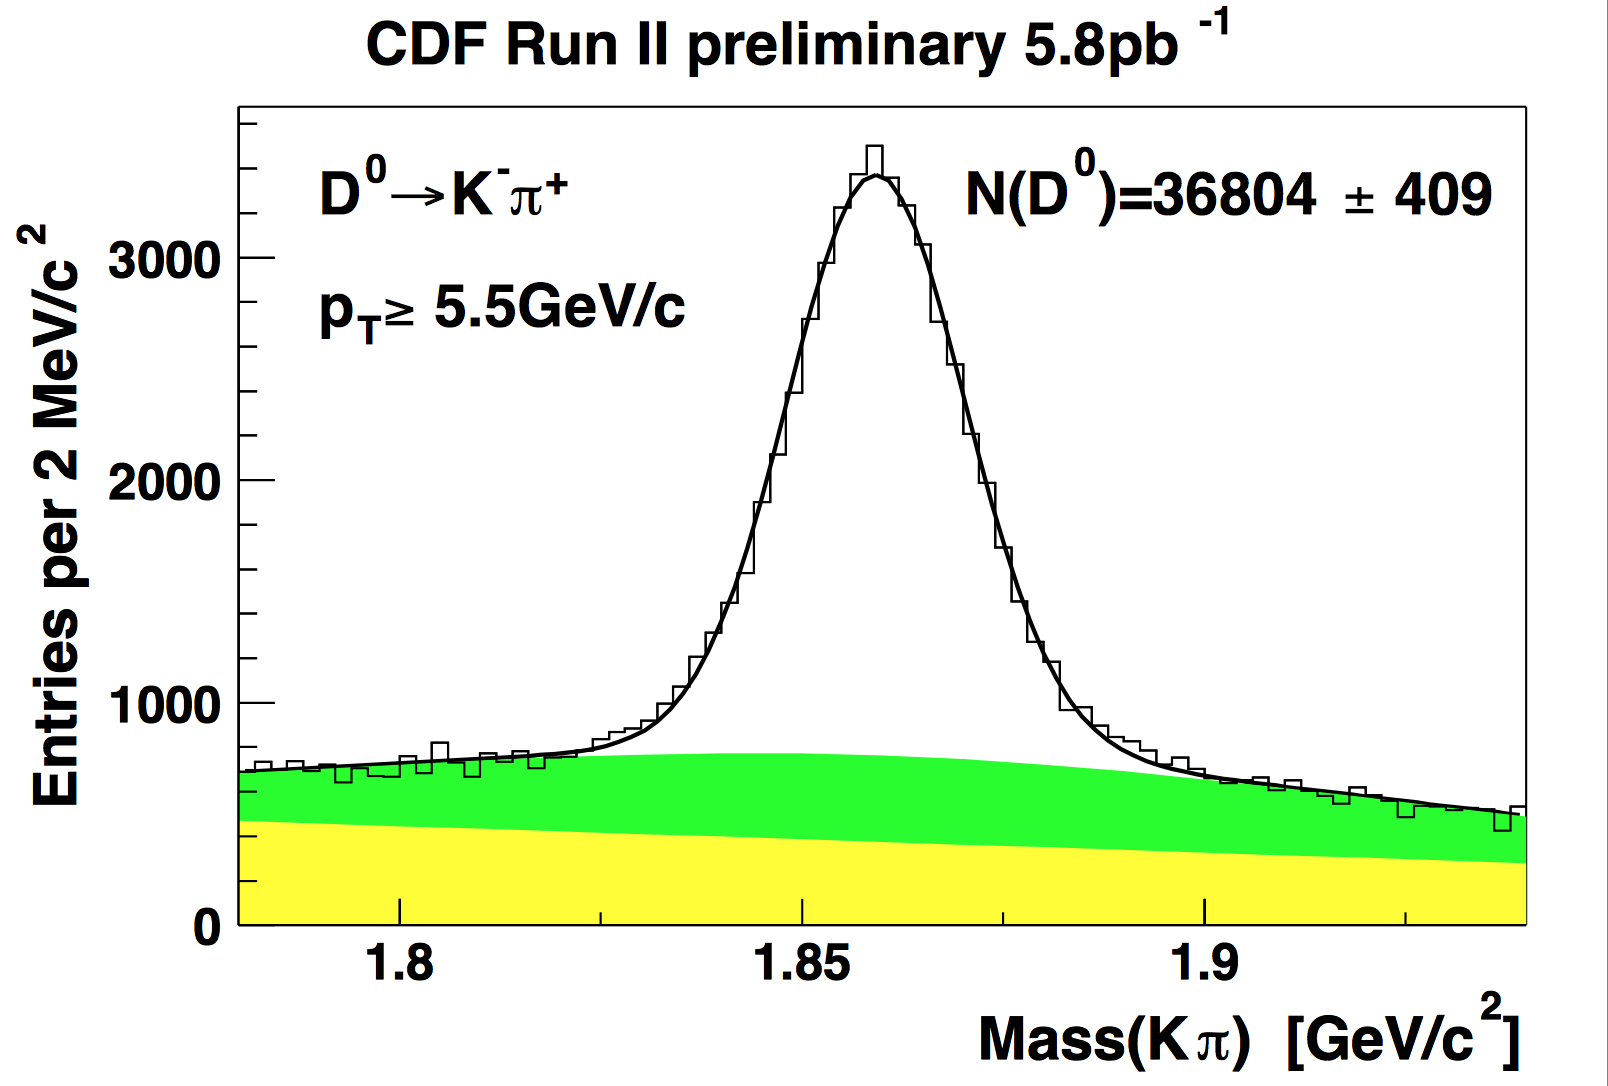
\includegraphics[scale=0.30]{CDF-Kpi}
\caption{\it $M_{K^+ \pi^-}$ invariant mass distribution from CDF.  The typical mass resolution is around 15 MeV here. \label{fig:Kpi}}
\end{figure}


\subsection{Step one: Identify the flavour/electrical charge of the Probe B meson using the trigger muon}
As the data sample will be triggered by the single muon trigger, it is possible to identify the electrical charge of the B meson, assuming it originates from a $B^+B^-$ production. Therefore, if the trigger muon possess a negative charge, we assume the probe B to be a $B^+$ and continue the reconstruction under this hypothesis. 

\subsection{Step two: Reconstruction of a $D^0 \rightarrow K^+ \pi^-$ candidate}
The next step in the reconstruction chain is to identify the best $D^0 \rightarrow K^+ \pi^-$ candidate in the event. The following criteria can help to accomplish this:
\begin{itemize}
\item [i)]  Identify opposite-sign pairs of tracks that stem from a common vertex. 
\item [ii)]  Assume that the positive charged track is a Kaon and apply the corresponding mass hypothesis.
\item [iii)] Calculate the invariant mass $M_{K^+ \pi^-}$ and define the mass difference $M_{D} - M_{K^+ \pi^-} = 1.864~GeV - M_{K^+ \pi^-}$. An example of a $M_{K^+ \pi^-}$ distribution from CDF is shown in Figure~\ref{fig:Kpi}. 
\item[iv)] Chose the candidate in the event that minimises $1.864~GeV - M_{K^+ \pi^-}$. This will be the  $D^0$ candidate used for the $B^+$ reconstruction step. 
\end{itemize}

\subsection{Step three:  Reconstruction of a $B^{+} \rightarrow D^0 \pi^{+} \rightarrow K^{+}  \pi^{-} \pi^{+}$ candidate}
The final step in the reconstruction chain is to identify the best $B^{+} \rightarrow D^0 \pi^{+} \rightarrow K^{+}  \pi^{-} \pi^{+}$ candidate using the $D^0$ candidate defined in Step two.  The following criteria can help to accomplish this:
\begin{itemize}
\item [i)]  Identify all positively charged tracks that for with the $D^0$ candidate a common vertex. The simplest procedure would be to search for common vertex of the $K^{+}  \pi^{-}$ pair with another positively charged track. Alternatively, the $K^{+}  \pi^{-}$ pair that represents the $D^0$ candidate could be refitted using the $D^0$ mass hypothesis, which could improve the resolution. As a first step, it seems advisable to focus on the simpler "three track" common vertex procedure. 
\item [ii)] Use all pairs of $D^0 \pi^+$ that form a common vertex and calculate the invariant mass $M_{K^+ \pi^- \pi^+}$. Define the mass difference: $M_{B^+} - M_{K^+ \pi^- \pi^+} = 5.279~GeV - M_{K^+ \pi^- \pi^+}$.
\item [ii)] Chose the candidate in the event that minimises $ 5.279~GeV - M_{K^+ \pi^- \pi^+}$ and plot the distribution of $M_{K^+ \pi^- \pi^+}$.
\end{itemize}


\section{Potential PhD Thesis Subject: Measurements of Branching Fraction Ratios and CP-asymmetries in Suppressed $B^{+} \rightarrow (K^{-}  \pi^{+})_D~ \pi^{+}$ and $B^{+} \rightarrow (K^{-}  \pi^{+})_D~K^{+}$ decays}
 \begin{figure}[htb]
\centering
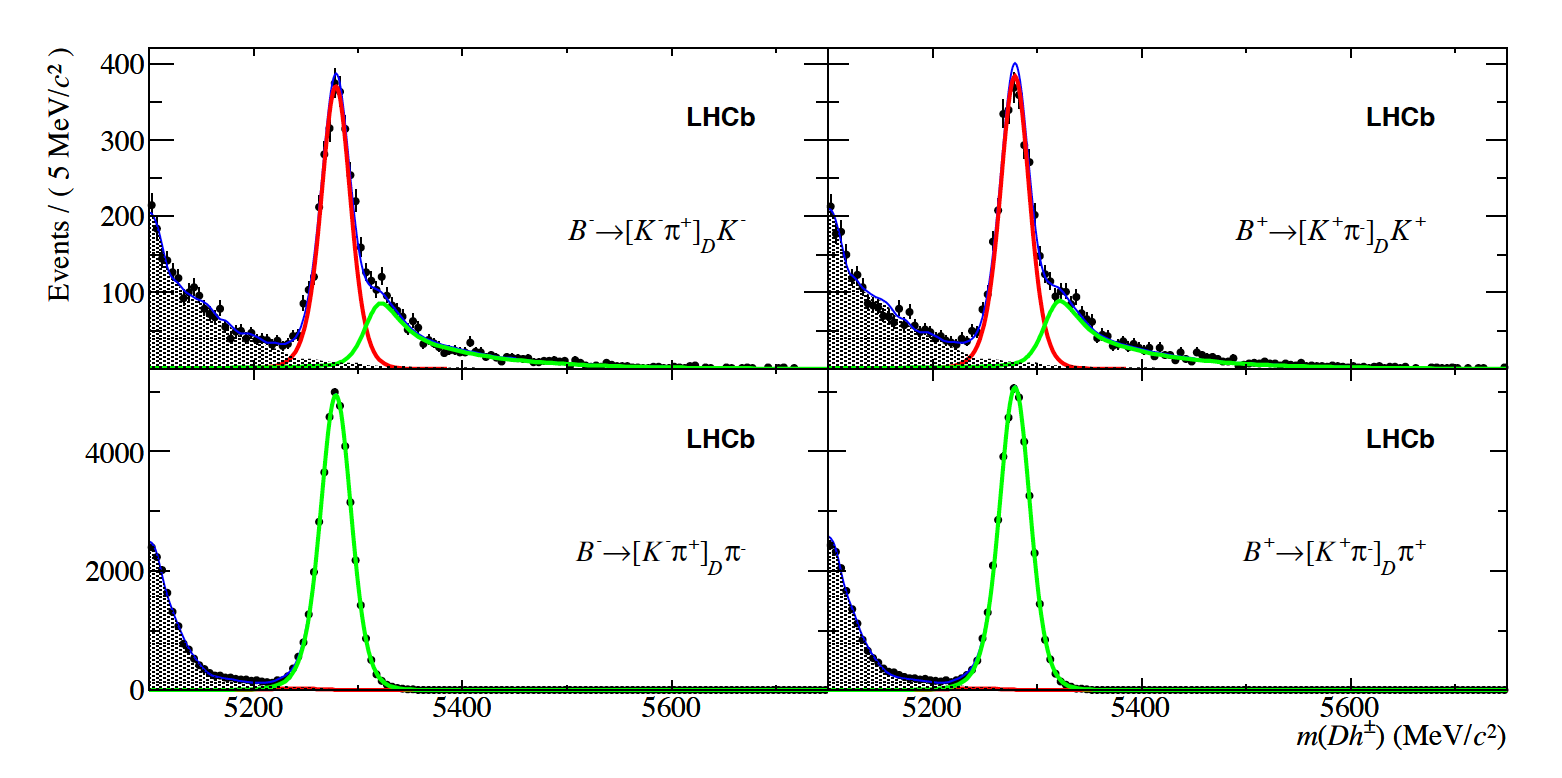
\includegraphics[scale=0.25]{LHCB-fav} 
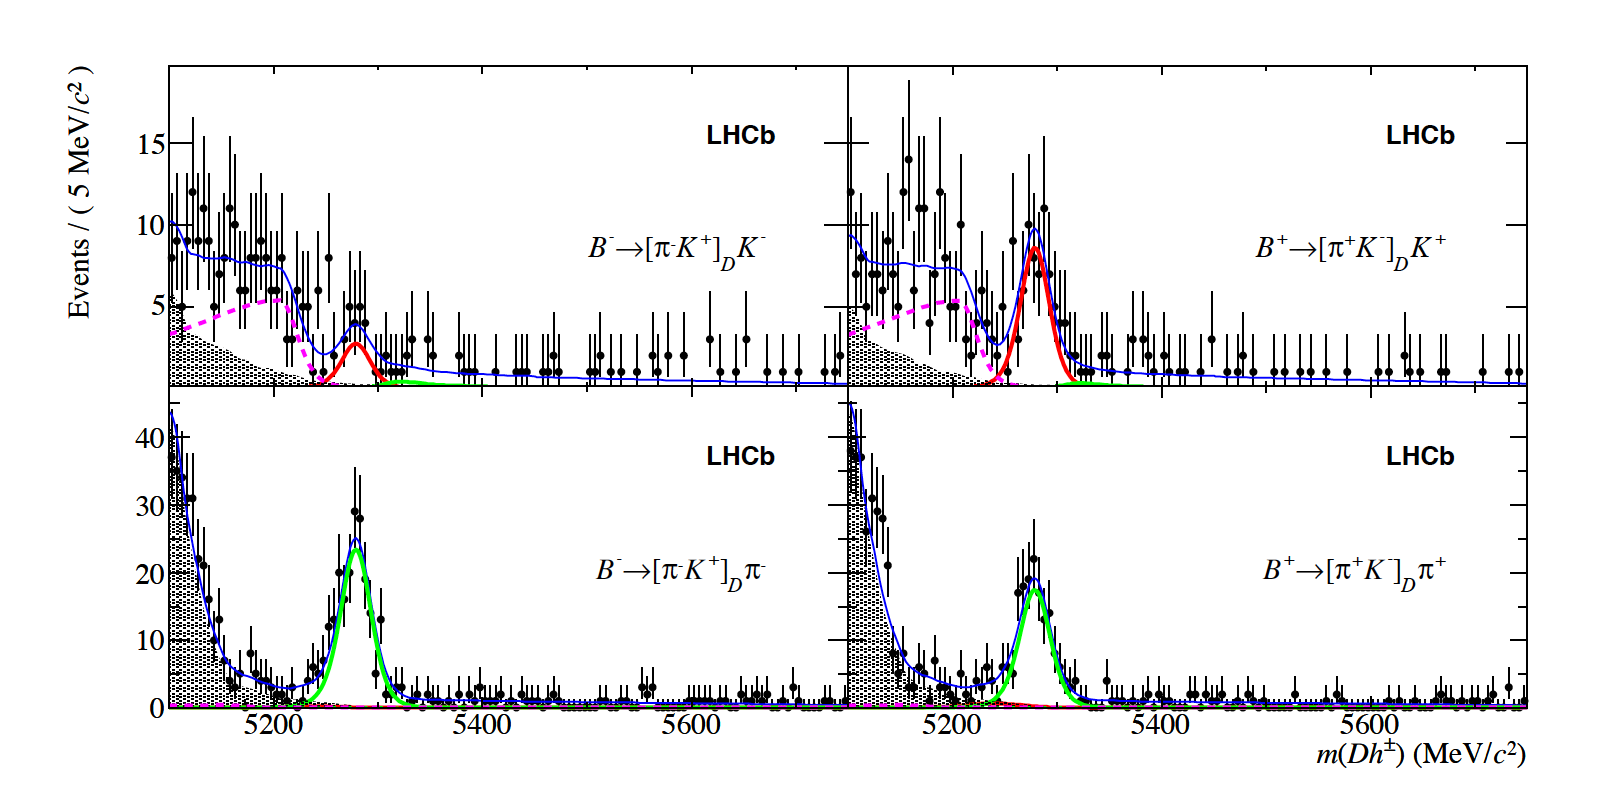
\includegraphics[scale=0.25]{LHCB-sup}
\caption{\it Invariant mass distributions of selected $ B \rightarrow  (K \pi)_D ~ h$ candidates from LHCb. The left four plots show $B^-$ and $B^+$ candidates for the favoured decay mode, while the four plots to the right show the suppressed decay mode. In the top plots, the bachelor track is identified to be a Kaon, while in the lower plots it is reconstructed as a pion. The dark (red) curve represents the  $B \rightarrow  (K \pi)_D ~ K$ events and the light (green) curve stands for $B \rightarrow  (K \pi)_D ~ \pi$  The shaded contribution are partially reconstructed events and the combinatorial component.\label{fig:lhcb}}
\end{figure}

In appendix~\ref{A} we have outlined how to reconstruct the  colour-favoured $B^{+} \rightarrow D^0 \pi^{+} \rightarrow K^{+}  \pi^{-} \pi^{+}$ decay. While this decay is important to perform a significant measurement of the B purity using the first reconstructed data, its suppressed counter-part $B^{+} \rightarrow (K^{-}  \pi^{+})_D~ \pi^{+}$ has more interesting physics to offer. In fact, the suppressed decays $B^{+} \rightarrow  (K^{-}  \pi^{+})_D~ \pi^{+}$ and $B^{+} \rightarrow (K^{-}  \pi^{+})_D~ K^{+}$ are sensitive to the CKM angle $\gamma$, which is a critical quantity in the unitarity triangle. 

\begin{table}[htb]
\label{tab:yields}
\footnotesize\center
\caption{\it Summary of the expected yields of important B modes that can be collected with 2~kHz of parking in 2018. For the 2018 we assume $sec_{\rm LHC}=7.8\times10^6$~\cite{scoutingW} of LHC running and $B$ hadron purity of $P_{\rm HLT}=0.8$ after a refinement of the L1 seed at the HLT (see Section~\ref{sub:L1}). Note that for the yield of $B^0\rightarrow K^*\ell^+\ell^-$ decays the factor $\frac{2}{3}$ for the decay of $K^*(893) \rightarrow K^{\pm} \pi^{\mp}$, which is required to fully reconstruct this decay, is already included. Note that the numbers in this table do not include the reconstruction efficiency.}
\vspace{0.1in}
\begin{tabular}{ |c|c|c|c| }
 \hline
Mode & $N_{2018}$ & $f_B$~\cite{FB} & ${\cal B}$   \\ \hline \hline 
\multicolumn{4}{|c|}{Suppressed and favoured $B^{+} \rightarrow D^0 h^{+}$ decays [h=K,$\pi$]} \\ \hline
$B^{+} \rightarrow (K^{+}  \pi^{-})_D^{fav} ~ \pi^{+} $&    $8.9\times 10^{5}$& 0.4  & $1.78 \times 10^{-4}$ \cite{PDG0}  \\ \hline
$B^{+}  \rightarrow (K^{-}  \pi^{+})_D^{sup}~ \pi^{+}$ &   $3140$& 0.4  & $6.3\times 10^{-7}$ \cite{PDG0}  \\ \hline \hline
$B^{+} \rightarrow (K^{+}  \pi^{-})_D^{fav}~ K^{+}$ &    $\approx 8 \times 10^{4}$& 0.4  & $\approx 1.5 \times 10^{-5}$ \cite{PDG0}  \\ \hline
$B^{+}  \rightarrow (K^{-}  \pi^{+})_D^{sup}~ K^{+} $&   $\approx 1500 $& 0.4  & $\approx 3 \times 10^{-7}$ \cite{PDG0}  \\ \hline \hline
\multicolumn{4}{|c|}{$R_K^{(*)}$} \\ \hline
$B^0\rightarrow K^* \ell^+\ell^-$ &   3290 & 0.4  & $\frac{2}{3} \times 9.9 \times 10^{-7}$ \cite{PDG0}  \\ \hline
$B^{\pm}\rightarrow K^{\pm} \ell^+\ell^-$ &  2250  & 0.4  & $4.51\times 10^{-7}$ \cite{PDG+}  \\ \hline
 \end{tabular}
\end{table}

As outlined in~\cite{Atwood:1996ci}, a powerful strategy to measure the angle $\gamma$ in tree-level processes is to study CP-violating observables in the decays $B^{+} \rightarrow D~h^{+}$  where D indicates a neutral charm meson which decays in a mode common to both $D^0$ and $\bar{D}^0$ states, and $h$, the bachelor hadron, is either a kaon or a pion. In the case of  $B^{+} \rightarrow D~h^{+}$, interference occurs between the suppressed $b\rightarrow u \bar{c} s$ and favoured $b\rightarrow c \bar{u} s$ decay paths, and similarly for the charge conjugate decay.  

Measuring  the suppressed decays of $B^{+} \rightarrow  (K^{-}  \pi^{+})_D^{sup}~ h^{+}$, with $h=\pi, K$ and normalising it to the favoured decay scenarios yields the following ratios: 

\[R_{Dh} = \frac{B^{+} \rightarrow  (K^{-}  \pi^{+})_D^{sup}~ h^{+}}{B^{+} \rightarrow  (K^{+}  \pi^{-})_D^{fav}~ h^{+}}. \]

An attempt to measure these ratios was carried out in~\cite{Aaij:2012kz, Aaltonen:2011uu, Saigo:2004de} but due to limited statistic, especially in the $B^{+} \rightarrow D~K^{+}$ final state, the results are not very significant yet. The latest result is is from LHCb~\cite{Aaij:2012kz} and the corresponding distributions are shown in Figure~\ref{fig:lhcb}.  While a few hundred events of the suppressed decay $B^{+} \rightarrow  (K^{-}  \pi^{+})_D^{sup}$ are observed, the suppressed decay with the kaon as bachelor track in the final state only shows a very weak signal.    
 

As shown in Table~ \ref{tab:yields}, the expected yields before acceptance and reconstruction efficiency for the suppressed $B \rightarrow  (K \pi)_D ~ h$ decays are similar to the one of $B^0\rightarrow K^* \ell^+\ell^-$ and $B^{\pm}\rightarrow K^{\pm} \ell^+\ell^-$. However, in contrast to the signal events of the $R_K^{(*)}$ measurements, the $B \rightarrow  (K \pi)_D ~ h$ final state does not require an improvement of the low-momentum electron reconstruction and already with state-of-the-art CMS reconstruction tools it should be possible to reconstruct a competitive data set of the  suppressed $B \rightarrow  (K \pi)_D ~ h$ decays, especially in the $h=\pi$ scenario. 

Therefore, the measurement of  $R_{Dh}$ would provide a natural fall-back option for a PhD thesis in case the requirement improvements in the electron reconstruction for a significant  $R_K^{(*)}$  cannot be accomplished.  It would also be a straightforward continuation of the B purity measurement outlined in appendix~\ref{A} using the favoured decay.     


\section{Procedure for generic Monte Carlo samples generation using the CMS software and computing infrastructure}\label{A}

CAVEAT: The steps described here are to be taken as a generic example to produce a sample using 2017 conditions down to the MINIAOD format. Some tuning of the number of threads for instance may be required depending on the specificity of each sample, on the statistics to generate and on the availability of the Grid sites. Those are inspired by the steps outlined in the following twiki
\url{https://twiki.cern.ch/twiki/bin/viewauth/CMS/BPHMonteCarloContactInfo#Recipe_of_Private_MC_production}

\subsection{Step one: GEN-SIM step}

A so-called gen-fragment file, corresponding to the process to generate, is needed for this step. Examples of such files are available here
\url{https://github.com/oozcelik/Fragments/blob/master/}
If new processes not available here need to be generated, a new gen-fragment needs to be developed by the user.
Help can be provided for this by the BPH MC contact O. Ozcelik (ozlem.ozcelik@cern.ch).
The gen-fragment can potentially refer to a decay file, such as the ones available here
\url{https://github.com/oozcelik/GeneratorInterface-EvtGenInterface}

The setup to run the GEN-SIM step can be installed following the instructions below

\bigbreak
cmsrel CMSSW\_9\_3\_6

cd CMSSW\_9\_3\_6/src

cmsenv

mkdir -p Configuration/GenProduction/python

\# put the gen fragment in this directory

scram b -j 9

cmsDriver.py Configuration/GenProduction/python/BToKee\_13TeV-pythia8-evtgen\_cfi.py --fileout file:BToKee\_GEN-SIM.root --mc --eventcontent RAWSIM --datatier GEN-SIM --conditions 93X\_mc2017\_realistic\_v3 --beamspot Realistic25ns13TeVEarly2017Collision --step GEN,SIM --nThreads 1 --geometry DB:Extended --era Run2\_2017 --python\_filename step1\_BToKee\_GEN-SIM\_cfg.py --no\_exec --customise Configuration/DataProcessing/Utils.addMonitoring -n 50

\bigbreak

Configuration/GenProduction/python/BToKee\_13TeV-pythia8-evtgen\_cfi.py is to be replaced by the proper gen-fragment file.
BToKee\_GEN-SIM.root and step1\_BToKee\_GEN-SIM\_cfg.py are arbitrary names for the output root files and the python script to be generated.
The python script can then be run using the standard crab submission on the grid.


\subsection{Step two: PUMIX step}

A different release is a priori needed to run this step. The following instructions can be followed to generate the corresponding python script.

\bigbreak
cmsrel CMSSW\_9\_4\_4

cd CMSSW\_9\_4\_4/src

cmsenv

scram b -j 9

cmsDriver.py --mc --eventcontent PREMIXRAW --datatier GEN-SIM-RAW --conditions 94X\_mc2017\_realistic\_v12 --step DIGIPREMIX\_S2,DATAMIX,L1,DIGI2RAW,HLT:2e34v40 --nThreads 4 --datamix PreMix --era Run2\_2017 --filein file:BToKee\_GEN-SIM.root --fileout file:BToKee\_PUMix.root --python\_filename step2\_BToKee\_PUMix\_cfg.py --pileup\_input /store/mc/RunIISummer17PrePremix/Neutrino\_E-10\_gun/GEN-SIM-DIGI-RAW/MC\_v2\_94X\_mc2017\_realistic\_v9-v1/30042/98009154-F2CD-E711-A4E1-FA163EC18760.root --no\_exec -n -1
\bigbreak

The python script can then be run using the standard crab submission on the grid.


\subsection{Step three: AODSIM step}

The same release as for the previous step can be used. The following instructions can be followed to generate the corresponding python script.

\bigbreak
cmsDriver.py --filein file:BToKee\_PUMix.root --fileout file:BToKee\_AODSIM.root --mc --eventcontent AODSIM runUnscheduled --datatier AODSIM --conditions 94X\_mc2017\_realistic\_v12 --step RAW2DIGI,RECO,RECOSIM,EI --nThreads 4 --era Run2\_2017 --python\_filename step3\_BToKee\_AODSIM\_cfg.py --no\_exec --customise Configuration/DataProcessing/Utils.addMonitoring -n -1
\bigbreak

The python script can then be run using the standard crab submission on the grid.


\subsection{Step four: MINIAODSIM step}

The same release as for the previous step can be used. The following instructions can be followed to generate the corresponding python script.

\bigbreak
cmsDriver.py --mc --eventcontent MINIAODSIM --runUnscheduled --datatier MINIAODSIM --conditions 94X\_mc2017\_realistic\_v12 --step PAT --era Run2\_2017 --filein file:BToKee\_AODSIM.root --fileout file:BToKee\_MINIAODSIM.root --python\_filename step4\_BToKee\_MINIAODSIM\_cfg.py --no\_exec -n -1
\bigbreak

The python script can then be run using the standard crab submission on the grid.


\subsection{Step five: NANOAOD step}

Dedicated plugins have been developed to store the relevant variables needed to perform the analysis, within the generic NANOAOD format recently adopted by CMS.
The corresponding code is maintained on the following git repository
\url{https://github.com/ICBPHCMS/cmssw}

\bigbreak
cmsrel CMSSW\_9\_4\_6\_patch1

cd CMSSW\_9\_4\_6\_patch1/src

cmsenv

git cms-merge-topic cms-nanoAOD:master100Xbase

git cms-merge-topic ICBPHCMS:NanoAOD\_BPH\_101X

scram b -j 4

cmsDriver.py test94X -s NANO --mc --eventcontent NANOAODSIM --datatier NANOAODSIM --filein /store/mc/RunIIFall17MiniAOD/TTToSemiLeptonic\_TuneCP5\_PSweights\_13TeV-powheg-pythia8/MINIAODSIM/94X\_mc2017\_realistic\_v10-v1/60000/A0D71AEE-13E1-E711-B3C9-FA163E629498.root --no\_exec  --conditions auto:phase1\_2017\_realistic -n 1000 --era Run2\_2017,run2\_nanoAOD\_94XMiniAODv1
\bigbreak

The python script can then be run using the standard crab submission on the grid.




%%%%%%%%%%%%%%%%%%%%%%%%%%
\bibliography{note.bib}
\bibliographystyle{JHEP}

\end{document}
%%%%%%%%%%%%%%%%%%%%%%%%%%%%%%%%%%%%%%%%%


